\documentclass[12pt]{report}
\usepackage[fontsize=13pt]{scrextend}
\usepackage[utf8]{vietnam}
\usepackage[utf8]{inputenc}
\usepackage[vietnamese]{babel}
\usepackage[sort, numbers]{natbib}
\usepackage[left=3cm,right=2cm,top=2.5cm,bottom=3cm]{geometry}
\usepackage{graphicx}

\title{sis}
\author{phamngocquy97 }
\date{February 2019}

\usepackage{natbib}
\usepackage{graphicx}

\begin{document}
	
%-----MAIN-----%
\newpage
\pagenumbering{arabic}
\setcounter{page}{1}
\chapter{Đặt vấn đề}
\chapter{Kiến thức cơ sở}
\chapter{Phương pháp kiểm tra sự tuân thủ mẫu thiết kế cho dự án sử dụng Java}
\newpage
Mẫu thiết kế là tập hợp các luật nhằm mô tả cách giải quyết một vấn đề trong thiết kế có thể là vấn đề lặp lại nhiều lần trong dự án. Với những dự án công nghệ thông tin nói chung và dự án Java nói riêng. Ở các mẫu thiết kế hướng đối tượng, thường thể hiện mối quan hệ giữa các lớp, các đối tượng với nhau. \\\\
Phương pháp ở đây dựa trên phấn tích tĩnh mã nguồn, bởi vì việc phân tích mã nguồn tĩnh đem lại độ chính xác tốt và quá trình phân tích không bắt buộc mã nguồn có thể thực thi được. Do đó dữ liệu đầu vào có thể là một phần hay toàn bộ mã nguồn của dự án.\\\\
Hình 3.1 mô tả phương pháp kiểm tra sự tuân thủ mẫu thiết kế. Đầu tiên, dữ liệu đầu vào được tiền xử lý thành cây cấu trúc, thông qua cây cấu trúc tiến hành phân tích phụ thuộc bên trong mã nguồn, xây dựng đồ thị phụ thuộc. Phân tích đồ thị phụ thuộc của mã nguồn và đồ thị phụ thuộc của mẫu thiết kế  nhằm kiểm tra sự tuân thủ mẫu thiết kế của mã nguồn.
\begin{figure}[h]
	\centering
	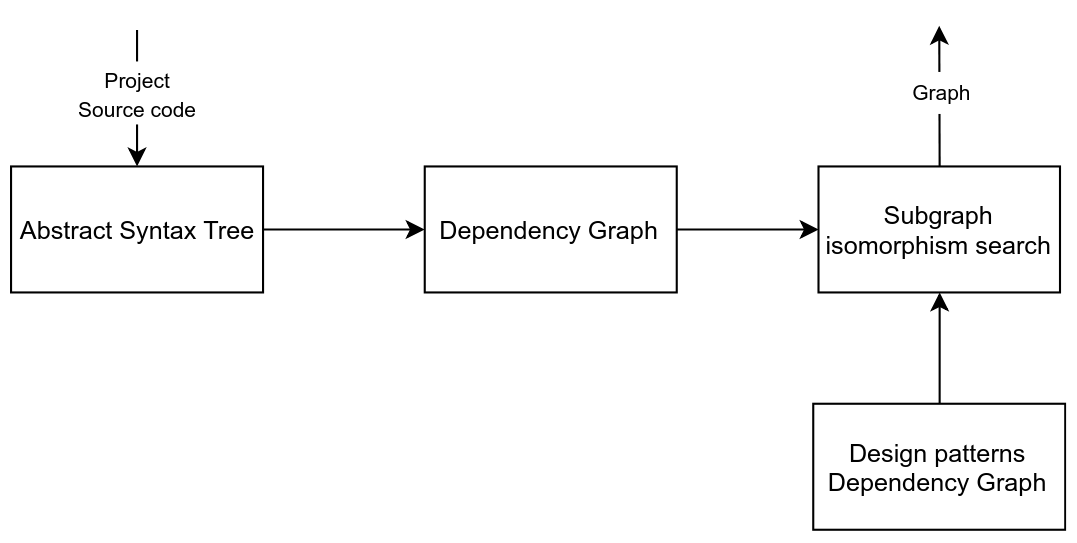
\includegraphics[scale=0.36]{images/general_architecture_3_1}
	\caption{Quá trình kiểm tra sự tuân thủ mẫu thiết kế của mã nguồn}
	\label{fig:general_architecture}
\end{figure}

\section{Tiền xử lý mã nguồn Java}
\subsection{Xây dựng cây cấu trúc}
Đối với phương pháp kiểm tra sự tuân thủ mẫu thiết kế mà khóa luận đề xuất. Cần có một kiểu dữ liệu tường minh và thể hiện được toàn bộ cấu trúc của mã nguồn, trong khi đó mã nguồn của dự án là phức tạp và chưa nhiều thông tin không được dùng tới. Nếu dùng trực tiếp mã sẽ gây khó khăn trong quá trình giải quyết bài toán và ảnh hưởng tới hiệu năng của của công cụ được xây dựng. Do đó cần tiến hành tiền xử lý mã nguồn, xây dựng một kiểu cấu trúc dữ liệu phù hợp. Cây cấu trúc được để xuất như là một kiểu cấu trúc dữ liệu phù hợp nhất thể hiện được toàn bộ cấu trúc của mã nguồn dự án.
\\
\\
\textbf{Định nghĩa: }(\textit{Cây cấu trúc} \cite{jcia}) Là một đồ thị liên thông với $T = (N,E)$ trong đó $N = \{n_1,n_2,n_3...n_k \}$ là tập các nút trên cây đại diện cho tệp, lớp, phương thức, biến... $E = \{(e_i,e_j) | e_i \in N , e_j \in N \}$ mỗi cặp $e_ie_j$ là cặp hai đỉnh kề của đồ thị.\\\\
Mô tả phương pháp tiền xử lý mã nguồn:
\begin{figure}[h]
	\centering
	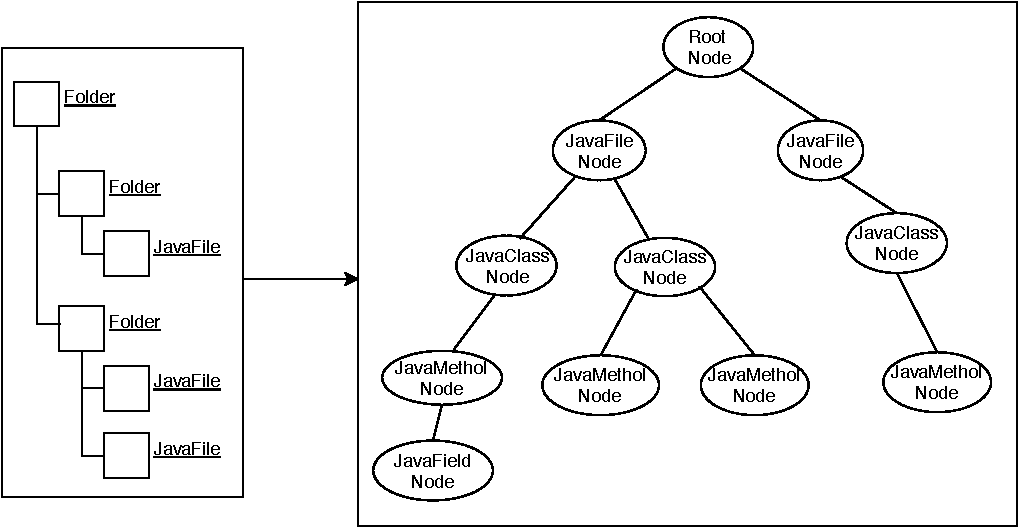
\includegraphics[scale=0.32]{images/structure_tree}
	\caption{Xây dựng cây cấu trúc từ mã nguồn}
	\label{fig:universe}
\end{figure}\\
Các nút trên cây được ánh xạ về bốn loại: tệp tin (\textit{Java}), lớp, phương thức và một loại nút thể hiện cho những định dạng còn lại. Mỗi loại nút của cây chứa những thuộc tính khác nhau và thông tin về nút cha, con của nó. Những thông tin trên mỗi nút được phân tích từ AST.
\subsection{Xác định thuộc tính cho mỗi nút trên cây cấu trúc}

Thành phần của một lớp gồm bốn phần chính: \textit{Class type, Class dependency, Class variables, Method }. Trong đó \textit{Class type} của một nút (class) thể hiện nút đó đóng vai trò như một:\textit{ Class, Abstract class, Template class} hay \textit{Interface}. \textit{Class depedency} ở đây  ta xét tới phụ thuộc thừa kế của lớp, phụ thuộc thừa kế bao gồm hai loại: kế thừa từ một class, kế thừa từ Interface. \textit{Method} là định nghĩa một hành vi của lớp, \textit{Method} bao gồm các thành phần: \textit{Local variable, Return type, Input paramater}  . \textit{Class variables} là biến của một lớp được khởi tạo bên ngoài các \textit{Method}. \textit{Local variable} là biến chỉ được khai báo và sử dụng trong phạm vi \textit{Method}. \textit{Return type} là kiểu dữ liệu mà phương thức sẽ trả về nếu \textit{Return type} là kiểu \textit{void} thì phương thức sẽ không trả về giá trị. \textit{Input paramter} xác định kiểu giá trị đầu vào cho phương thức.
\\\\
Hình 3.3 mô tả hai loại phụ thuộc kế thừa. Trong đó A là một Class thừa kế từ B là một Interface qua phương thức extend, C là một class thừa kế D qua phương thức implement với D là một abstract class.
\begin{figure}[h]
	\centering
	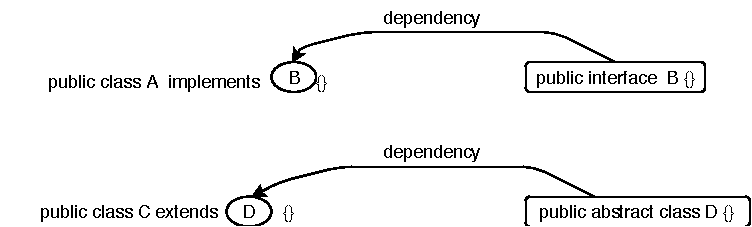
\includegraphics[scale=0.45]{images/class_dependency}
	\caption{Phụ thuộc thừa kế của lớp}
	\label{fig:dependecy_extend}
\end{figure}\\\\
Hình 3.4 Các thành phần cơ bản của \textit{Class}. Trong đó E là một Class với Access modifer là public, Class variable là sum với kiểu giá trị int, phương thức add có kiểu trả về là int và hai biến đầu vào là a và b.
\begin{figure}[h]
	\centering
	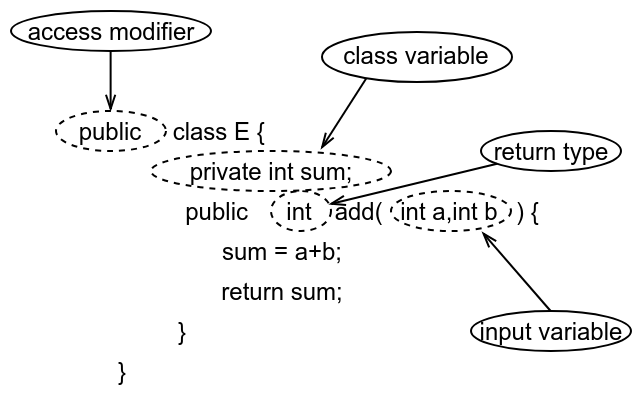
\includegraphics[scale=0.45]{images/class_method_structure}
	\caption{Các thành phần cơ bản trong class}
	\label{fig:class_structure}
\end{figure}
\newpage
Bảng 3.5 mô tả đầy đủ những thông tin cần xác định cho mỗi loại nút trên cây cấu trúc.\\
\begin{table}[h]
	\centering
	\tiny
	\renewcommand{\arraystretch}{1.6}
	\resizebox{1\textwidth}{!}{%
		\begin{tabular}{|p{2cm}|p{5cm}|}
			\hline
			\centering
			\textbf{Node} &  \multicolumn{1}{c|}{\textbf{Properties}} \\ \hline
			\centering
			Class & \begin{tabular}[c]{@{}l@{}}NameType\\ Access modifier\\ Extended Class\\ Implemented Class\\ Childrent Node: Field, Method\end{tabular} \\ \hline
			\centering
			Method & \begin{tabular}[c]{@{}l@{}}Name\\ NameReturn Type\\ Access modifier\\ Parameter\\ Body\end{tabular} \\ \hline
			\centering
			Field & \begin{tabular}[c]{@{}l@{}}Name\\ Value type\\ Access modifier\end{tabular} \\ \hline
		\end{tabular}%
	}
	\caption{Thuộc tính trên mỗi nút}
	\label{tab:node_properties}
\end{table}
\newpage
Trích xuất các thông tin từ mã nguồn cho các nút trên cây, được thực hiện thông qua AST. Với mỗi thành phần mã nguồn, ta sử dụng JP để sinh AST tương ứng với thành phần đó từ đó trích xuất các thuộc tính cần thiết cho mỗi nút trên cây cấu trúc. Hình 3.5 mô tả một AST với một Class Java tương ứng. Trong đó một lớp Java được phân tách thành dạng cây với các nút gốc chưa các toán tử, các nút lá chứa các toán hạng. Ví dụ như return = 42, với return là một toán tử ứng với n 'ReturnStatement' và '42' là toán hạng ứng với nút lá.
\begin{figure}[h]
	\centering
	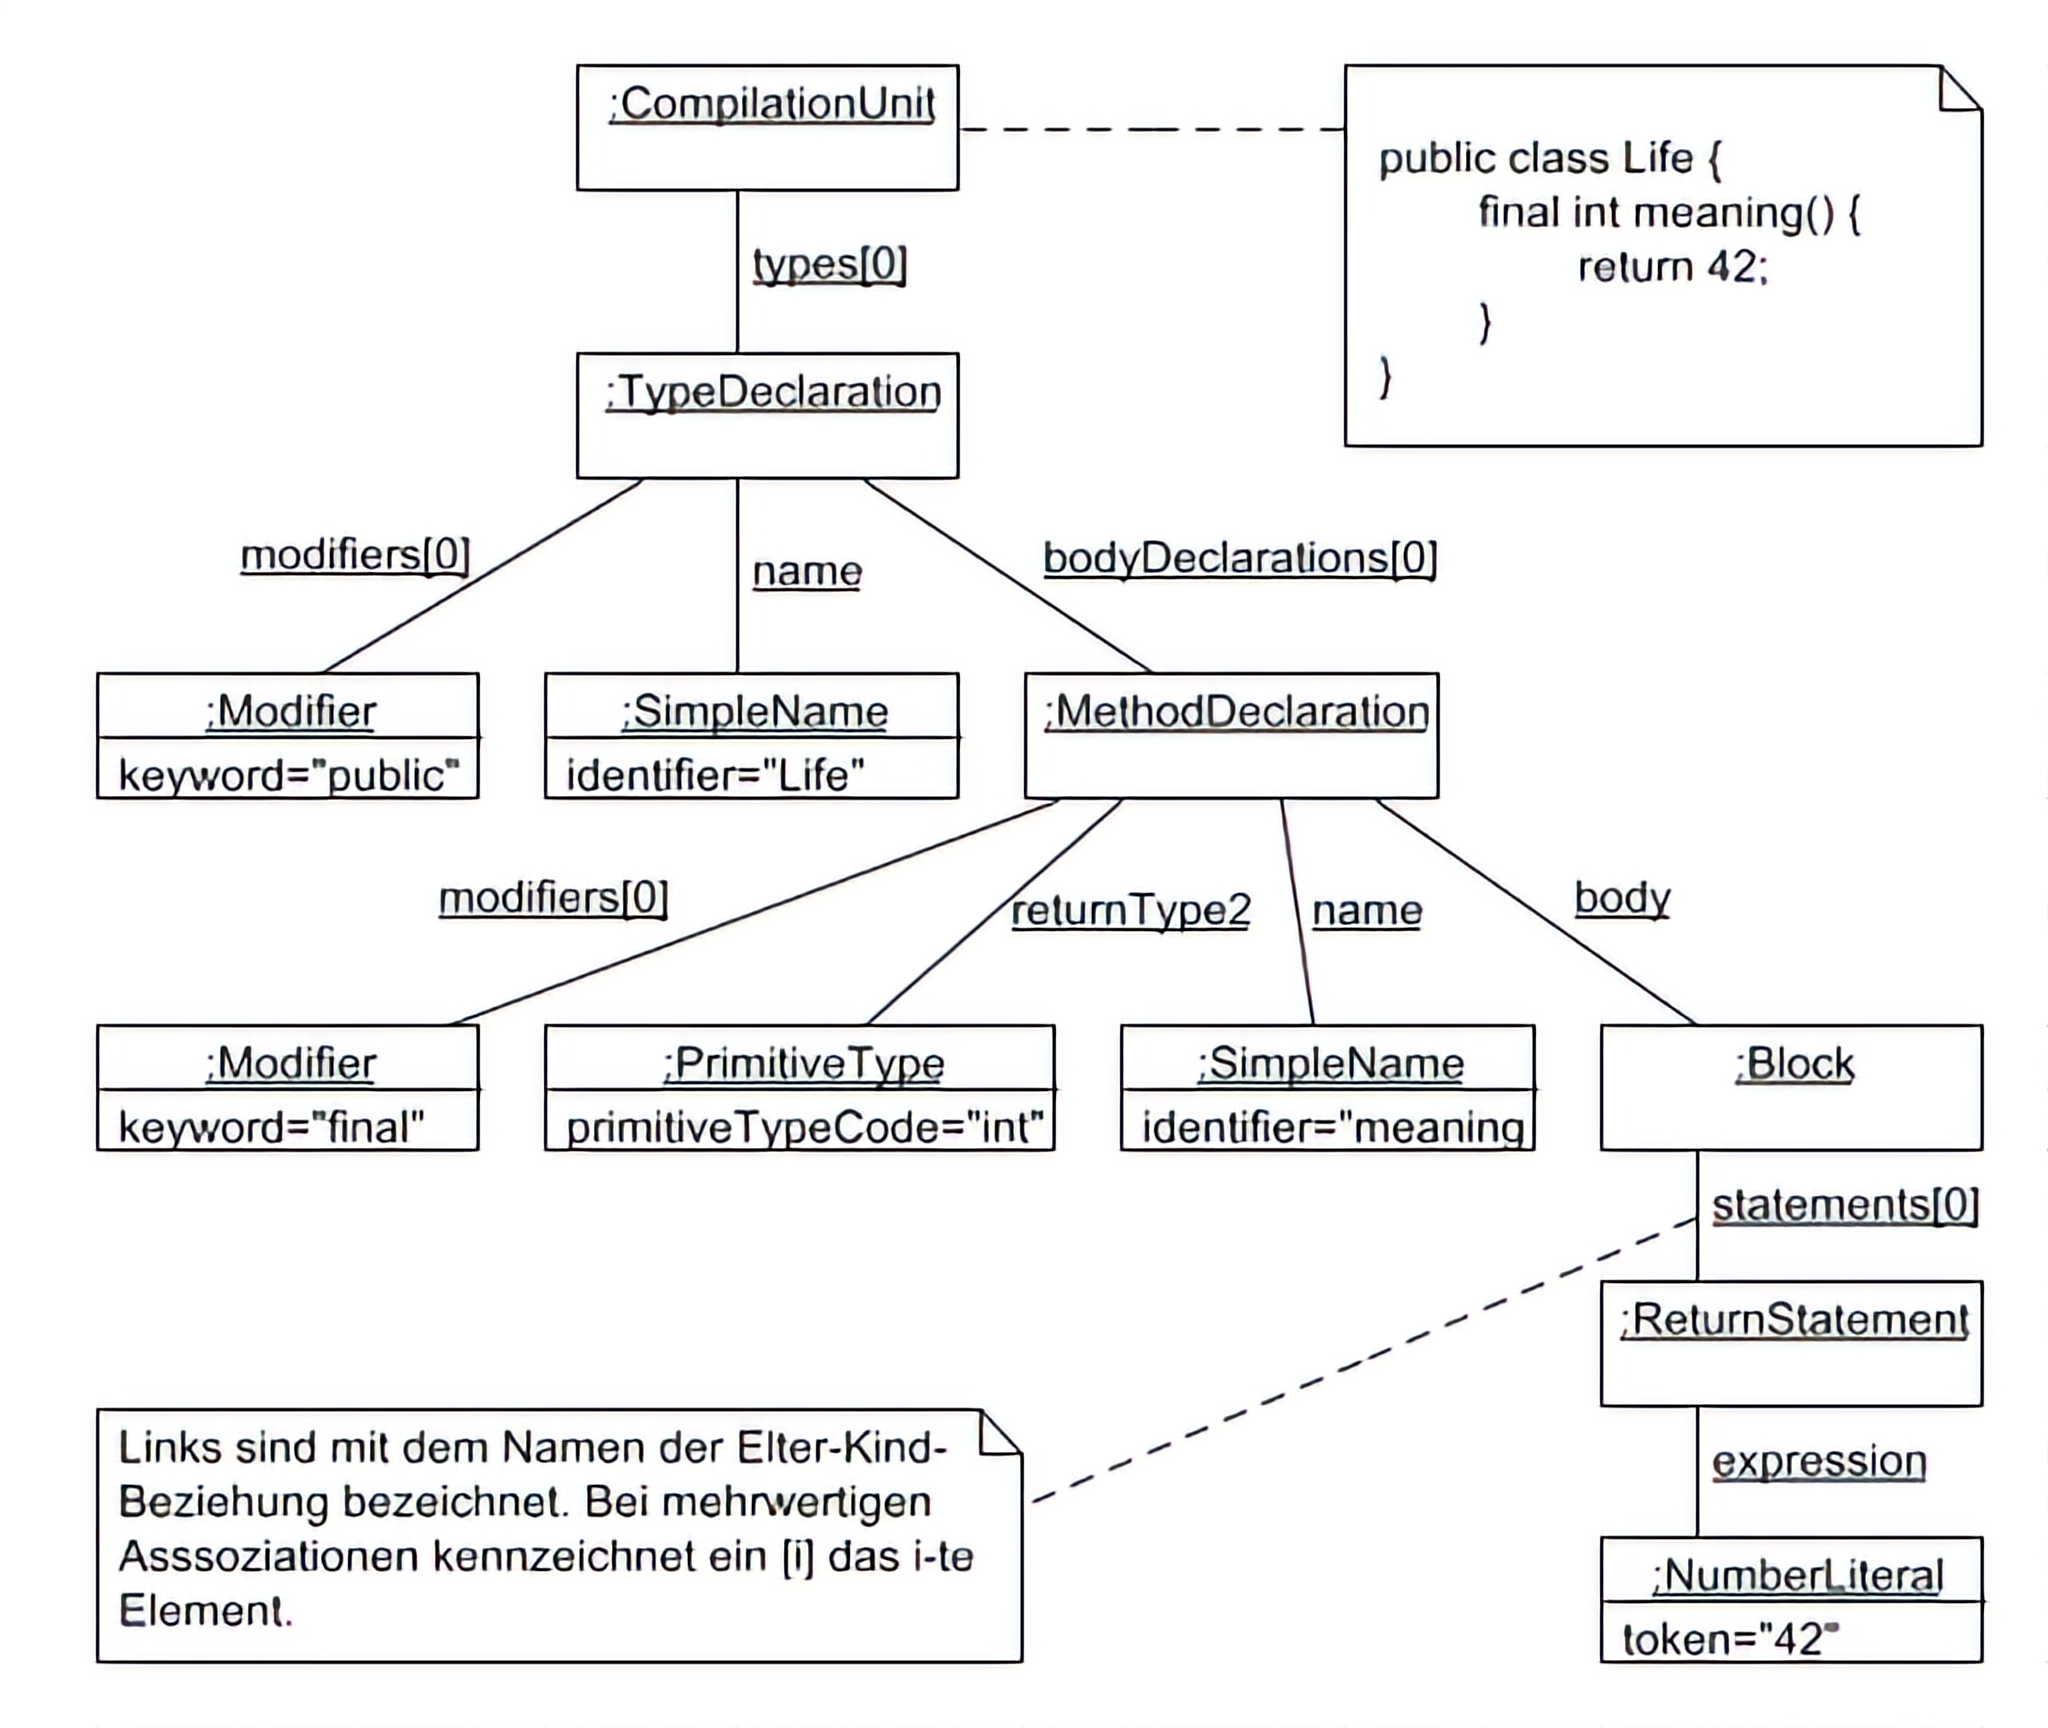
\includegraphics[scale=1]{images/ast_class_java-boring}
	\caption{Abstract syntax tree đối với Java class}
	\label{fig:ast_for_java_class}
\end{figure}\\

\newpage
\section{Phân tích cấu trúc mã nguồn Java}
Cấy cấu trúc thể hiện thể hiện chi tiết về cấu trúc của mã nguồn bao gồm các khía cạnh về tính hướng đối tượng bên trong mã nguồn. Phân tích cấu trúc mã nguồn nhằm xác định được những đặc điểm về mặt phụ thuộc giữa các thành phần mã nguồn được hình thành bới việc áp dụng những mẫu thiết kế bên trong mã nguồn. Xác định được những được những đặc nêu trên là tiền để để kiểm tra sự tuân thủ mẫu thiết kế bên trong mã nguồn.
\subsection{Phân tích phụ thuộc giữa các thành phần trong mã nguồn}
Đối với phương pháp mà khóa luận này đề xuất, việc phân tích phụ thuộc giữa các thành phân bên trong mã nguồn xoay quanh việc phân tích phụ thuộc giữa các lớp trong mã nguồn. Đối với loại phụ thuộc giữa các lớp trong mã nguồn Java bao gồm: Direct \& Indirect dependency, Polymorphism dependency, Inheritance Dependency.\\\\
\textbf{Polymorphism dependency}: Ở đây ta xem xét hai trường hợp của lọai pụụ thuộc này. Trường hợp thứ nhất khi một Class thừa kế một Interface bằng phương thức Implement. Ví dụ Class, A  thừa kế một interface B, Class A sẽ thừa kế những phương thức của Interface C, tức là tại Class A những phương thức được Interface C định nghĩa sẽ được triển khai. Ngoài ra tham chiếu của Interface B có thể trỏ tới đối tượng của Class A, trong trường hợp đó đối tượng tạo được trỏ tới bởi B chỉ có thể thực hiện những phương thức mà B đã định nghĩa, nhưng phương thúc khác của A sẽ bị làm mờ đi. Trường hợp thứ hai, phụ thuộc xảy ra khi một class thừa kế một class khác thông qua phương thức extends. Ví dụ, class C thừa thế class D, lúc này ta coi D như là Class cha, với C là class con, C sẽ thừa hưởng mọi thuộc tính và phương thức của  D, do đó C có thể ghi đè những phương thức của D, ngoài ra, tham chiếu của Class D có thể trỏ tới đối tượng của class C. Hình 3.6 và 3.7 mô tả ví dụ về hai trường hợp mà ta đã đề cập.
\begin{figure}[!htbp]
	\vspace*{-2cm}
	\centering
	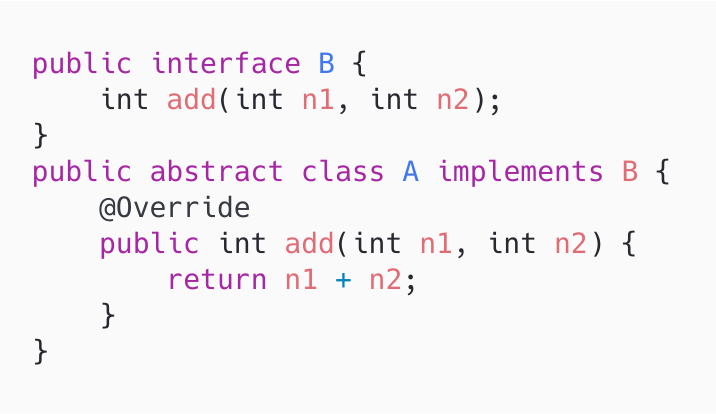
\includegraphics[scale=0.5]{images/AimplementsB}
	\caption{Mối quan hệ giữa một Class vớ một Interface qua phương thức Implements}
	\label{fig:A_implemets_B}
\end{figure}
\begin{figure}[!htbp]
	\centering
	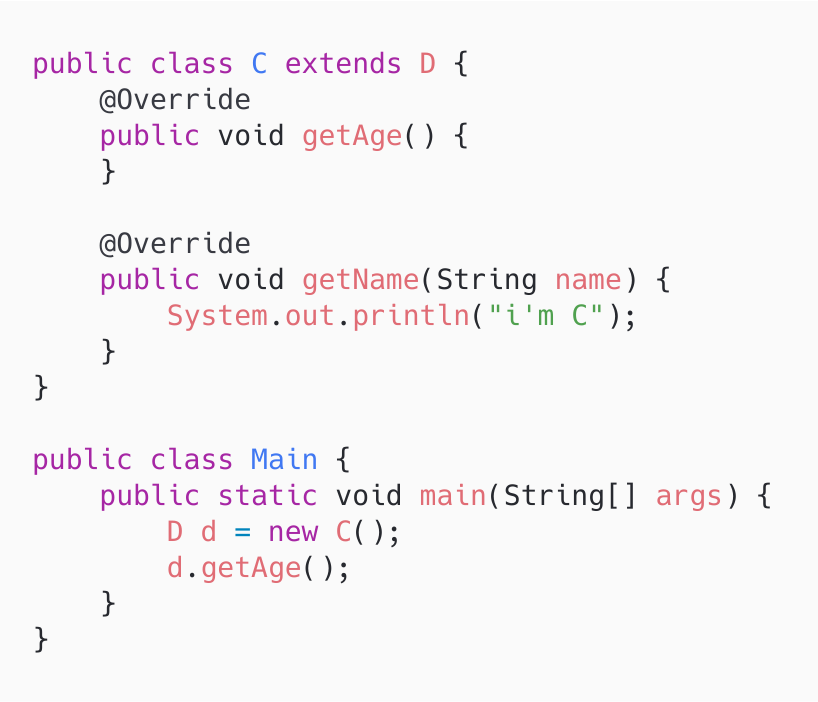
\includegraphics[scale=0.5]{images/CextendD}
	\caption{Mối quan hệ giữa một Class với một Class qua phương thức extends}
	\label{fig:CextendD}
\end{figure}



\pagebreak
\textbf{Inheritance Dependency}: Khi một Class có được các thuộc tính và phương thức của một Class khác. Những thuộc tính và phương thức này được quản lý theo thứ tự phân cấp từ lớp con tới lớp cha, việc xử lý phân cấp được quyết định trong quán trình chương trình đang thực thi bởi JVM. Ví dụ, ta có Class D thừa kế Class E với phương thức \textit{extends}, khi đó D sẽ thừa hưởng các phương thưc và thuộc tính của E. Trong trường hợp các phương thức và thuộc tính của D có \textit{Access modifier} là \textit{private}, khi đó đối tượng của Class A sẽ không thể gọi tới những thuộc tính, phương thức này. Hình 3.7 mô tả mối quan hệ thừa kết giữa hai Class Java.
\begin{figure}[!htbp]
	\centering
	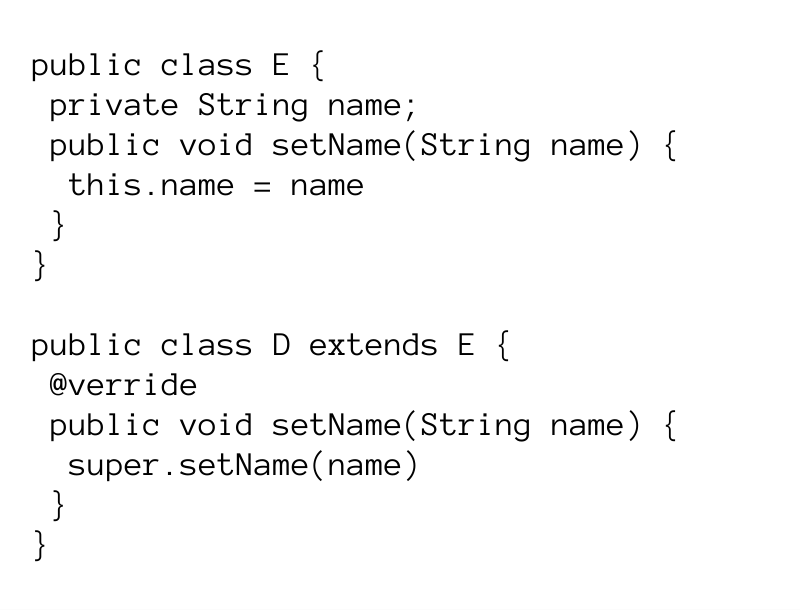
\includegraphics[scale=0.5]{images/D_extends_E}
	\caption{Mối quan hệ giữa một Class vớ một Interface qua phương thức Implements}
	\label{fig:D_extends_E}
\end{figure}\\\\
\textbf{Use Dependency}: 
\newpage
\subsection{Xây dựng đồ thị phụ thuộc từ cây cấu trúc}
\subsection{Ví dụ minh họa}
\section{Kiểm tra sự tuân thủ mẫu thiết kế bên trong mã nguồn}

\begin{thebibliography}{9}
	\section*{Tiếng Việt}
	\section*{Tiếng Anh}
	\bibitem{jcia}
	Hello latex	ia
	
	\bibitem{jp}
	Nicholas Smith, Danny van Bruggen, Federico Tomassetti
	JavaParser: Visited
	\textit{Analyse, transform and generate your Java code base}
\end{thebibliography}



\end{document}
